% !TEX program = xelatex
% ============================================================
%  TEMPLATE SKRIPSI POLITEKNIK STATISTIKA STIS
%  Prodi D-IV Komputasi Statistik  |  Pedoman Edisi Keenam (2025)
%
%  PENTING (Overleaf): Menu -> Settings -> Compiler -> "XeLaTeX".
%  Berkas latexmkrc sudah memaksa XeLaTeX + Biber bila pengaturan
%  menu tidak diubah. Jangan memakai pdfLaTeX.
% ============================================================
\documentclass[12pt,a4paper,twoside,openright,fleqn]{report}

\usepackage{skripsistis}        % seluruh format STIS (lihat skripsistis.sty)
\addbibresource{referensi.bib}  % basis data referensi (BibTeX)

% ------------------------------------------------------------
%  METADATA SKRIPSI (isi sesuai data Anda)
% ------------------------------------------------------------
% PEMINATAN: hilangkan tanda komentar baris berikut untuk Sistem Informasi
% Statistik (enam bab). Biarkan dikomentari untuk Sains Data (lima bab).
% \peminatansitrue
%
\judulskripsi{Pemodelan Proxy Means Test Berbasis GPBoost untuk Penargetan Kemiskinan}
\subjudulskripsi{}              % kosongkan bila tidak ada subjudul
\namamhs{Achmad Syahrul Choir}
\nimmhs{222212501}
\peminatan{Sains Data}          % atau: Sistem Informasi Statistik
\tahunskripsi{2026}
\tglsidang{[tanggal sidang]}
\pengujiI{Dr. Penguji Satu, M.Si.}      \nipPengujiI{0000}
\pengujiII{Dr. Penguji Dua, M.Si.}      \nipPengujiII{0000}
\ketuaprodi{Dr. Ketua Prodi, M.Si.}     \nipKetuaprodi{0000}
\pembimbing{Dr. Pembimbing, M.Si.}      \nipPembimbing{0000}

\begin{document}

% ====================== HALAMAN MUKA ========================
% ============================================================
%  Halaman muka: Sampul, Halaman Judul, Pernyataan, Pengesahan,
%  dan Lembar Hak Cipta. Isi diambil dari metadata di main.tex.
% ============================================================
\begin{titlepage}
\pagenumbering{gobble}
\singlespacing   % seluruh halaman muka diketik 1 spasi (kecuali blok yang diatur)
\centering

% Subjudul opsional (jarak antar baris sub judul 1,5 spasi; pedoman).
\newcommand{\skSubjudulBlok}{%
  \ifdefempty{\skSubjudul}{}{%
    \par\vspace{\spasi}%
    {\bfseries\fontsize{14}{21}\selectfont\skSubjudul\par}}%
}

% ---------- HALAMAN SAMPUL ----------
\vspace*{-0.7\spasi}  % kompensasi leading; judul mulai ~baris kedua
% Judul: kapital, TNR 14 pt, jarak antar baris 2 spasi (pedoman).
{\bfseries\fontsize{14}{28}\selectfont\MakeUppercase{\skJudul}\par}
\skSubjudulBlok

% Jarak Nama dengan baris terakhir judul/sub judul = 5 spasi (pedoman).
\vspace{5\spasi}
% Nama & NIM: kapital, TNR 12 pt, jarak Nama-NIM 1,5 spasi (pedoman).
{\bfseries\fontsize{12}{18}\selectfont%
  \MakeUppercase{\skNama}\\ \skNIM\par}

% Jarak Program Studi dengan NIM = 4,5 spasi (pedoman).
\vspace{4.5\spasi}
% Program Studi & Peminatan: TNR 12 pt, blok di TENGAH (nilai membungkus).
{\bfseries\fontsize{12}{12}\selectfont
\begin{tabular}{@{}l@{\hspace{0.6em}}c@{\hspace{0.6em}}>{\raggedright\arraybackslash}p{6.7cm}@{}}
\textbf{PROGRAM STUDI} & : & \textbf{KOMPUTASI STATISTIK PROGRAM DIPLOMA IV} \\
\textbf{PEMINATAN}     & : & \textbf{\MakeUppercase{\skPeminatan}} \\
\end{tabular}\par}

\vfill
% Logo 5 cm x 5 cm, simetris antara Program Studi dan tulisan STIS (pedoman).
\IfFileExists{img/logo_stis.png}{
\includegraphics[width=5cm,height=5cm,keepaspectratio]{img/logo_stis.png}\par}{\rule{0pt}{5cm}\par}
\vfill

% Tiga baris terakhir: kapital, TNR 14 pt, jarak antar baris 1,5 spasi (pedoman).
{\bfseries\fontsize{14}{21}\selectfont%
  POLITEKNIK STATISTIKA STIS\\ JAKARTA\\ \skTahun\par}
\clearpage

% ---------- HALAMAN JUDUL ----------
\thispagestyle{empty}
\centering
\vspace*{-0.7\spasi}
% Judul: format sama dengan halaman sampul.
{\bfseries\fontsize{14}{28}\selectfont\MakeUppercase{\skJudul}\par}
\skSubjudulBlok

% Tulisan SKRIPSI berjarak 5 spasi setelah baris terakhir judul/sub judul (pedoman).
\vspace{5\spasi}
{\bfseries\fontsize{12}{12}\selectfont SKRIPSI\par}
% "Diajukan sebagai ..." jarak antar baris 1,5 spasi (pedoman).
\vspace{\spasi}
{\bfseries\fontsize{12}{18}\selectfont%
  Diajukan sebagai Salah Satu Syarat untuk Memperoleh Sebutan\\
  Sarjana Terapan Statistika pada Politeknik Statistika STIS\par}

% "Oleh:" pada baris ketiga (3 spasi) setelah tulisan sebelumnya (pedoman).
\vspace{3\spasi}
{\bfseries\fontsize{12}{12}\selectfont Oleh:\par}
{\bfseries\fontsize{12}{18}\selectfont%
  \MakeUppercase{\skNama}\\ \skNIM\par}

\vfill
\IfFileExists{img/logo_stis.png}{
\includegraphics[width=5cm,height=5cm,keepaspectratio]{img/logo_stis.png}\par}{\rule{0pt}{5cm}\par}
\vfill

{\bfseries\fontsize{14}{21}\selectfont%
  POLITEKNIK STATISTIKA STIS\\ JAKARTA\\ \skTahun\par}
\clearpage

% ---------- HALAMAN PERNYATAAN ----------
% Catatan: tanggal pada halaman ini = TANGGAL SIDANG/UJIAN AKHIR.
\thispagestyle{empty}
\begin{center}{\bfseries\large PERNYATAAN}\end{center}
\vspace{0.8cm}
\begin{center}
{\bfseries Skripsi dengan Judul\par}
\vspace{0.4cm}
{\bfseries \MakeUppercase{\skJudul}\par}
\ifdefempty{\skSubjudul}{}{{\bfseries \skSubjudul\par}}
\end{center}
\vspace{1.2cm}

\begin{center}
Oleh:\\[0.2cm]
\textbf{\MakeUppercase{\skNama}}\\
\textbf{\skNIM}
\end{center}
\vspace{1.2cm}

\noindent\justifying adalah benar-benar hasil penelitian sendiri dan bukan hasil plagiat
atau hasil karya orang lain. Jika di kemudian hari diketahui ternyata skripsi ini hasil
plagiat atau hasil karya orang lain, penulis bersedia skripsi ini dinyatakan tidak sah
dan sebutan Sarjana Terapan Statistika dicabut atau dibatalkan.
\vspace{1.5cm}

\begin{flushright}
\begin{minipage}{7cm}\centering
Jakarta, \skTglSidang\ \skTahun\\[2.2cm]
\textbf{\skNama}
\end{minipage}
\end{flushright}
\clearpage

% ---------- HALAMAN PENGESAHAN ----------
\thispagestyle{empty}
\begin{center}{\bfseries\large \MakeUppercase{\skJudul}}\end{center}
\ifdefempty{\skSubjudul}{}{\begin{center}{\bfseries \skSubjudul}\end{center}}
\vspace{0.6cm}
\begin{center}Oleh:\\[0.2cm]\textbf{\MakeUppercase{\skNama}}\\ \textbf{\skNIM}\end{center}
\vspace{0.8cm}

\begingroup
\small
\newcommand{\ttdblok}[3]{% #1 jabatan, #2 nama (bold), #3 NIP
  \begin{minipage}[t]{0.5\textwidth}\centering
  \begin{minipage}[t][2.2\baselineskip][t]{\linewidth}\centering #1\end{minipage}\\[2cm]
  \textbf{#2}\\
  NIP #3
  \end{minipage}%
}

\begin{center}\normalsize\textbf{Tim Penguji}\end{center}
\vspace{0.2cm}
\noindent
\ttdblok{Penguji I}{\skPengujiI}{\skNIPpengujiI}\hfill
\ttdblok{Penguji II}{\skPengujiII}{\skNIPpengujiII}
\vspace{1cm}

\begin{center}\normalsize Mengetahui/Menyetujui\end{center}
\vspace{0.2cm}
\noindent
\ttdblok{Ketua Program Studi\\Komputasi Statistik Program Diploma IV}{\skKaprodi}{\skNIPkaprodi}\hfill
\ttdblok{Pembimbing}{\skPembimbing}{\skNIPpembimbing}
\endgroup
\clearpage

% ---------- LEMBAR HAK CIPTA ----------
\thispagestyle{empty}
\vspace*{\fill}
\begin{center}
\fbox{%
  \begin{minipage}{0.78\textwidth}
  \itshape
  \setlength{\parindent}{0pt}
  \vspace{0.5\baselineskip}
  {\bfseries \textcopyright\ Hak Cipta milik Politeknik Statistika STIS, Tahun \skTahun}

  \vspace{0.5\baselineskip}
  {\bfseries Hak Cipta dilindungi undang-undang}
  \begin{enumerate}[leftmargin=*,labelsep=0.5em,topsep=0.3\baselineskip,itemsep=0.2\baselineskip]
    \item Dilarang mengutip sebagian atau seluruh karya tulis, hasil analisis,
          perancangan, basis data, program, dan artefak hasil skripsi ini tanpa
          mencantumkan atau menyebutkan sumbernya.
      \begin{enumerate}[label=\alph*.,leftmargin=1.5em,labelsep=0.5em,topsep=0.2\baselineskip,itemsep=0.2\baselineskip]
        \item Pengutipan hanya untuk kepentingan pendidikan, penelitian, penulisan
              karya ilmiah, penyusunan laporan, penulisan kritik atau tinjauan suatu
              masalah.
        \item Pengutipan tidak merugikan kepentingan yang wajar Politeknik Statistika
              STIS.
      \end{enumerate}
    \item Dilarang mengumumkan dan memperbanyak sebagian atau seluruh karya tulis,
          hasil analisis, perancangan, basis data, program, dan artefak hasil skripsi
          ini dalam bentuk apa pun tanpa seizin Politeknik Statistika STIS.
  \end{enumerate}
  \vspace{0.3\baselineskip}
  \end{minipage}%
}
\end{center}
\vspace*{\fill}
\clearpage
\end{titlepage}
   % sampul, judul, pernyataan, pengesahan, hak cipta

% Bagian awal: angka Romawi kecil, dimulai dari Prakata, di tengah bawah.
% Di bagian awal, setiap bagian cukup pindah halaman (tanpa sisipan halaman
% kosong); penyisipan "halaman kosong" hanya berlaku untuk bab isi (openright).
\pagenumbering{roman}
\setcounter{page}{1}
\let\skClearDouble\cleardoublepage
\let\cleardoublepage\clearpage

% ---------- PRAKATA ----------
\chapter*{Prakata}
\addcontentsline{toc}{chapter}{PRAKATA}

Puji syukur penulis panjatkan ke hadirat Tuhan Yang Maha Esa atas selesainya
skripsi ini. Skripsi berjudul ``\skJudul'' disusun sebagai salah satu syarat
untuk memperoleh sebutan Sarjana Terapan Statistika pada Politeknik Statistika STIS.

Pada kesempatan ini penulis menyampaikan terima kasih kepada semua pihak yang telah
membantu, antara lain:
\begin{enumerate}[leftmargin=*]
  \item Dosen pembimbing atas arahan dan bimbingannya;
  \item Tim penguji atas masukan yang membangun;
  \item keluarga dan rekan-rekan atas dukungannya.
\end{enumerate}

Penulis menyadari skripsi ini masih memiliki kekurangan. Kritik dan saran yang
membangun sangat penulis harapkan. Semoga skripsi ini bermanfaat.

\vspace{1cm}
\begin{flushright}
\begin{minipage}{6cm}\centering
Jakarta, \skTahun\\[1.5cm]
Penulis
\end{minipage}
\end{flushright}

% ---------- ABSTRAK ----------
% Jumlah halaman "x+N" dihitung otomatis: x = halaman romawi terakhir,
% N = halaman isi terakhir (lihat \label{akhirfront} & paket lastpage).
\chapter*{Abstrak}
\addcontentsline{toc}{chapter}{ABSTRAK}
\begin{spacing}{1.5}
\noindent\textbf{\skNama}, ``\skJudul''.\par
\noindent\pageref{akhirfront}+\pageref{LastPage} halaman\par
\vspace{0.5\baselineskip}

\noindent\justifying
Abstrak berisi ringkasan skripsi yang dideskripsikan secara jelas, padat, dan
singkat, dengan maksimum 200 kata. Isi abstrak terdiri atas permasalahan
penelitian, deskripsi metode/sistem yang dikembangkan, hasil evaluasi, kesimpulan,
dan saran. Abstrak ditulis dalam satu atau dua paragraf, diketik 1,5 spasi, serta
menghindari sitasi dan singkatan tak baku.
\vspace{0.5\baselineskip}

\noindent\textbf{Kata Kunci:} \hangindent=2.2cm kata kunci pertama, kata kunci kedua,
kata kunci ketiga, hingga maksimum enam kata kunci.
\end{spacing}


% Daftar-daftar (masing-masing didaftarkan ke Daftar Isi & DI HALAMAN TERPISAH)
\clearpage
\addcontentsline{toc}{chapter}{DAFTAR ISI}
\tableofcontents
\clearpage
\addcontentsline{toc}{chapter}{DAFTAR TABEL}
\listoftables
\clearpage
\addcontentsline{toc}{chapter}{DAFTAR GAMBAR}
\listoffigures
\clearpage
\addcontentsline{toc}{chapter}{DAFTAR LAMPIRAN}
\listoflampiran

% Daftar Singkatan & Simbol (OPSIONAL -- hapus dua baris ini bila tak diperlukan)
% ---------- DAFTAR SINGKATAN (opsional) ----------
% Hapus \input berkas ini di main.tex bila tidak diperlukan.
\judulfrontmatter{Daftar Singkatan}{DAFTAR SINGKATAN}
\begin{singlespace}
\noindent\begin{tabularx}{\textwidth}{@{}p{3cm}X@{}}
\textbf{Singkatan} & \textbf{Keterangan} \\[2pt]
\hline \\[-8pt]
BPS    & Badan Pusat Statistik \\
PMT    & \emph{Proxy Means Test} \\
Susenas & Survei Sosial Ekonomi Nasional \\
\end{tabularx}
\end{singlespace}

% ---------- DAFTAR SIMBOL (opsional) ----------
% Hapus \input berkas ini di main.tex bila tidak diperlukan.
\judulfrontmatter{Daftar Simbol}{DAFTAR SIMBOL}
\begin{singlespace}
\noindent\begin{tabularx}{\textwidth}{@{}p{3cm}X@{}}
\textbf{Simbol} & \textbf{Keterangan} \\[2pt]
\hline \\[-8pt]
$\alpha$      & taraf nyata (tingkat signifikansi) \\
$\beta$       & koefisien regresi \\
$\hat{y}$     & nilai dugaan (prediksi) peubah respons \\
$\mu$         & rata-rata (mean) populasi \\
$\sigma$      & simpangan baku (standar deviasi) populasi \\
\end{tabularx}
\end{singlespace}


% Penanda akhir bagian awal (untuk hitung "x+N halaman" pada Abstrak).
\clearpage
\label{akhirfront}

% ======================= BAGIAN ISI =========================
% Bagian isi: angka Arab, dimulai dari 1, di kanan bawah (pedoman).
% Pulihkan perilaku openright (bab isi mulai di halaman ganjil/kanan).
\let\cleardoublepage\skClearDouble
\cleardoublepage
\aktifkanNomorIsi
\pagenumbering{arabic}
\setcounter{page}{1}
\doublespacing                 % teks isi diketik 2 spasi (pedoman hlm. 34)

\chapter{Pendahuluan}

\section{Latar Belakang}
Kemiskinan merupakan fakta sosial global yang selalu menjadi perhatian dari tahun
ke tahun \parencite{megawati2021}. Salah satu metode standar untuk mengidentifikasi
penerima program bantuan sosial adalah \emph{Proxy Means Test} (PMT)
\parencite{etang2022}. \textcite{taufiq2021} menunjukkan bahwa pendekatan
\emph{ensemble} dapat meningkatkan akurasi penargetan.

% (Uraikan konteks, kesenjangan, dan posisi penelitian Anda di sini.)

\section{Identifikasi dan Batasan Masalah}
Bagian ini memuat identifikasi masalah dan batasan ruang lingkup penelitian.

\section{Tujuan Penelitian}
Bagian ini memuat tujuan penelitian yang ingin dicapai.

\section{Manfaat Penelitian}
Bagian ini memuat manfaat teoretis dan praktis dari penelitian.

\section{Sistematika Penulisan}
\ifpeminatansi
Penulisan skripsi ini terdiri atas enam bab. Bab I Pendahuluan menguraikan latar
belakang, identifikasi dan batasan masalah, tujuan, manfaat, serta sistematika
penulisan. Bab II Tinjauan Pustaka memuat landasan teori dan penelitian terkait.
Bab III Metode Penelitian menjelaskan data serta metodologi pengembangan sistem
yang digunakan. Bab IV Analisis dan Perancangan menyajikan analisis kebutuhan dan
rancangan sistem. Bab V Implementasi dan Evaluasi memaparkan implementasi sistem
beserta hasil pengujian dan evaluasinya. Bab VI Kesimpulan dan Saran berisi
kesimpulan penelitian dan saran untuk pengembangan selanjutnya.
\else
Penulisan skripsi ini terdiri atas lima bab. Bab I Pendahuluan menguraikan latar
belakang, identifikasi dan batasan masalah, tujuan, manfaat, serta sistematika
penulisan. Bab II Tinjauan Pustaka memuat landasan teori dan penelitian terkait.
Bab III Metode Penelitian menjelaskan data, tahapan, dan teknik analisis yang
digunakan. Bab IV Hasil dan Pembahasan menyajikan temuan penelitian beserta
pembahasannya. Bab V Kesimpulan dan Saran berisi kesimpulan penelitian dan saran
untuk penelitian selanjutnya.
\fi

% Catatan: paragraf di atas mengikuti penanda \peminatansi (lihat main.tex).

\chapter{Tinjauan Pustaka}

\section{Landasan Teori}
Bagian ini memuat teori yang menjadi dasar penelitian. Konsep dan sifat formal
dapat dinyatakan dengan lingkungan definisi, teorema, dan bukti berbahasa Indonesia.

\begin{definisi}[Proxy Means Test]
Misalkan $y_i$ menyatakan log pengeluaran per kapita rumah tangga ke-$i$ dan
$\mathbf{x}_i$ vektor karakteristik teramati. \emph{Proxy Means Test} adalah fungsi
prediksi $\hat{f}:\mathbf{x}_i \mapsto \hat{y}_i$ yang diperoleh dengan meminimumkan
suatu fungsi galat $\sum_i L\!\left(y_i,\hat{f}(\mathbf{x}_i)\right)$.
\end{definisi}

\begin{teorema}\label{teo:ols}
Pada model linear $y = \mathbf{X}\beta + \varepsilon$ dengan
$\mathrm{E}(\varepsilon \mid \mathbf{X}) = \mathbf{0}$, penduga kuadrat terkecil
$\hat{\beta} = (\mathbf{X}^\top\mathbf{X})^{-1}\mathbf{X}^\top y$ bersifat takbias.
\end{teorema}

\begin{proof}
Substitusi $y = \mathbf{X}\beta + \varepsilon$ memberikan
$\hat{\beta} = \beta + (\mathbf{X}^\top\mathbf{X})^{-1}\mathbf{X}^\top\varepsilon$.
Karena $\mathrm{E}(\varepsilon \mid \mathbf{X}) = \mathbf{0}$, maka
$\mathrm{E}(\hat{\beta} \mid \mathbf{X}) = \beta$.
\end{proof}

\section{Penelitian Terkait}
Beberapa penelitian terdahulu mengembangkan PMT dengan pendekatan
\emph{machine learning} \parencite{etang2022,taufiq2021}.

\section{Penulisan Kutipan}
Format sitasi mengikuti APA versi 7 dengan penyesuaian bahasa Indonesia
(\emph{dan} untuk dua pengarang, \emph{dkk.} untuk lebih dari dua pengarang,
\emph{hal.} untuk halaman).

\subsection{Kutipan Tidak Langsung (Parafrase)}
Kutipan tidak langsung mencantumkan nama pengarang dan tahun \emph{tanpa} nomor
halaman. Satu pengarang: \textcite{cochran1991} memformalkan teori penarikan
sampel. Dua pengarang: \textcite{taufiq2021} membandingkan beberapa algoritma.
Lebih dari dua pengarang: \textcite{etang2022} menekankan pentingnya validasi
silang. Versi dalam kurung berturut-turut: \parencite{cochran1991};
\parencite{taufiq2021}; \parencite{etang2022}.

\subsection{Kutipan Langsung Pendek (kurang dari atau sama dengan 40 kata)}
Kutipan langsung pendek diberi tanda kutip serta nomor halaman. Naratif (nomor
halaman di akhir kutipan): \textcite{cochran1991} menyatakan bahwa ``penarikan
sampel acak sederhana memberikan estimasi takbias bagi rata-rata populasi''
(hal.~10). Dalam kurung: ``replikasi data memungkinkan akses yang konsisten
lintas waktu'' \parencite[hal.~781]{taufiq2021}.

\subsection{Kutipan Langsung Panjang (lebih dari 40 kata)}
Kutipan langsung panjang ditulis pada paragraf tersendiri, menjorok 1 tab dari
batas kiri teks, tanpa tanda kutip:
\begin{kutipanpanjang}
Proxy means testing merupakan pendekatan yang banyak dipakai untuk menargetkan
bantuan sosial ketika data pendapatan rumah tangga tidak tersedia atau sulit
diverifikasi; metode ini menaksir kesejahteraan dari sejumlah peubah proksi yang
mudah diamati, sehingga keputusan penargetan dapat dilakukan secara lebih objektif
dan dapat direplikasi \parencite[hal.~25]{etang2022}.
\end{kutipanpanjang}

\subsection{Mengutip dari Kutipan (Sitasi Sekunder)}
Diperbolehkan bila pustaka asli sulit ditemukan: nama pengarang asli dicantumkan
pada kalimat, sumber sekunder (tempat kutipan ditemukan) pada akhir kalimat.
Menurut Nelder dan Wedderburn (1972), seperti dikutip dalam
\textcite{cochran1991}, prinsip estimasi takbias menjadi dasar banyak metode
inferensi. Pada Daftar Pustaka hanya dicantumkan sumber sekunder yang
benar-benar dibaca (Cochran), bukan sumber asli (Nelder dan Wedderburn).

\subsection{Sitasi Lembaga/Instansi Pemerintah}
Bila penulis berupa lembaga/instansi, pada \textbf{kemunculan pertama} ditulis
nama lengkap diikuti akronim, lalu \textbf{kemunculan selanjutnya} cukup akronim
(pedoman 4.4). Pada entri bib: \verb|author = {{Badan Pusat Statistik}}| (kurung
ganda agar tidak dipenggal) dan \verb|shortauthor = {BPS}|.

Kemunculan pertama (naratif): \textcite{bps2024} menetapkan garis kemiskinan
secara nasional. Dalam kurung: \parencite{bps2024}. Kemunculan selanjutnya cukup
akronim: \textcite{bps2024}, atau \parencite{bps2024}. Pada Daftar Pustaka, nama
lembaga \emph{selalu} ditulis lengkap (Badan Pusat Statistik), bukan akronim.

\subsection{Sitasi Direktorat di Bawah Kementerian}
Bila karya disusun oleh suatu \textbf{direktorat di bawah kementerian}, ikuti
APA-7: unit \textbf{paling spesifik menjadi penulis}, kementerian induk menjadi
\textbf{penerbit} (jangan menggabung keduanya sebagai satu nama). Pada entri bib:
\verb|author = {{Direktorat Jenderal Pembangunan Desa dan Perdesaan}}|,
\verb|shortauthor = {Ditjen PDP}|, dan \verb|institution = {Kementerian ...}|.

Kemunculan pertama: \textcite{ditjenpdp2023} menyusun pedoman alokasi dana desa.
Selanjutnya: \textcite{ditjenpdp2023}; atau dalam kurung \parencite{ditjenpdp2023}.
Pada Daftar Pustaka, nama direktorat (penulis) diikuti judul, lalu kementerian
sebagai penerbit.

\ifpeminatansi
  % --- Peminatan SISTEM INFORMASI STATISTIK (enam bab) ---
  \chapter{Metode Penelitian}
\emph{Cara menulis bab ini.} Bab Metode Penelitian (Sistem Informasi) menjelaskan data/kebutuhan, metodologi pengembangan sistem, serta alat dan bahan. Uraikan cukup rinci agar dapat direplikasi.


\section{Data dan Kebutuhan Sistem}
\emph{Cara menulis.} Uraikan kebutuhan fungsional dan non-fungsional sistem serta data yang digunakan.

Bagian ini menjelaskan sumber data (mis.\ basis data BPS) serta kebutuhan sistem
yang akan dikembangkan.

\section{Metodologi Pengembangan Sistem}
\emph{Cara menulis.} Jelaskan metodologi yang dipilih (mis.\ \emph{Waterfall}, \emph{Prototyping}, \emph{Agile}) beserta tahapannya.

Pengembangan sistem mengikuti pendekatan \emph{System Development Life Cycle}
(SDLC) dengan model \emph{prototyping}. Tahapan pengembangan disajikan pada
Gambar~\ref{gbr:sdlc}.

\begin{figure}[H]
\centering
\begin{tikzpicture}[node distance=0.95cm]
  \node[fc-mulai] (a) {Komunikasi/Analisis Kebutuhan};
  \node[fc-proses, below=of a] (b) {Perancangan Cepat (Prototipe)};
  \node[fc-proses, below=of b] (c) {Pembangunan Prototipe};
  \node[fc-putusan, below=of c] (d) {Diterima?};
  \node[fc-proses, below=of d] (e) {Implementasi \& Pengujian};
  \draw[fc-panah] (a)--(b); \draw[fc-panah] (b)--(c); \draw[fc-panah] (c)--(d);
  \draw[fc-panah] (d)-- node[right]{ya} (e);
  \draw[fc-panah] (d.west) -- ++(-2.2,0) |- node[pos=0.25,left]{tidak} (b.west);
\end{tikzpicture}
\caption{Tahapan pengembangan sistem dengan model prototyping}
\label{gbr:sdlc}
\end{figure}

\section{Alat dan Bahan}
\emph{Cara menulis.} Sebutkan perangkat keras/lunak, bahasa, dan \emph{framework} yang digunakan.

Perangkat lunak dan pustaka yang digunakan, antara lain bahasa pemrograman,
kerangka kerja (\emph{framework}), dan sistem manajemen basis data.

  \chapter{Analisis dan Perancangan}
\emph{Cara menulis bab ini.} Bab Analisis dan Perancangan menyajikan analisis kebutuhan dan rancangan sistem (proses, basis data, dan antarmuka).


\section{Analisis Kebutuhan}
\emph{Cara menulis.} Identifikasi kebutuhan fungsional dan non-fungsional berdasarkan rumusan masalah.

Analisis kebutuhan dibagi menjadi kebutuhan fungsional dan nonfungsional.
Kebutuhan fungsional sistem dirangkum pada Tabel~\ref{tab:fungsional}.

\begin{table}[H]
\centering
\caption{Kebutuhan fungsional sistem}
\label{tab:fungsional}
\begin{tabular}{|c|l|}
\hline
\textbf{Kode} & \textbf{Kebutuhan Fungsional} \\ \hline
\multicolumn{1}{|c|}{(1)} & \multicolumn{1}{c|}{(2)} \\ \hline
KF-01 & Sistem dapat melakukan autentikasi pengguna. \\
KF-02 & Sistem dapat mengunggah dan memvalidasi data. \\
KF-03 & Sistem dapat menampilkan hasil prediksi. \\ \hline
\end{tabular}
\end{table}

\section{Perancangan Proses (Use Case)}
\emph{Cara menulis.} Gambarkan proses dengan \emph{use case}/diagram alir beserta deskripsinya.

Interaksi pengguna dengan sistem digambarkan pada \emph{use case diagram}
Gambar~\ref{gbr:usecase}.

\begin{figure}[H]
\centering
\begin{tikzpicture}
  \node (sys) [uc-sistem, minimum width=5cm, minimum height=4cm] at (2.2,0) {};
  \node[above] at (sys.north) {\small Sistem};
  \pic (akt) at (-2.2,0) {uc-aktor};
  \node[below] at (-2.2,-1.2) {\small Pengguna};
  \node[uc-case] (u1) at (2.2,1.2) {Login};
  \node[uc-case] (u2) at (2.2,0)   {Unggah Data};
  \node[uc-case] (u3) at (2.2,-1.2){Lihat Prediksi};
  \draw[uc-asosiasi] (-2.0,0) -- (u1);
  \draw[uc-asosiasi] (-2.0,0) -- (u2);
  \draw[uc-asosiasi] (-2.0,0) -- (u3);
\end{tikzpicture}
\caption{Use case diagram sistem}
\label{gbr:usecase}
\end{figure}

\section{Perancangan Basis Data}
\emph{Cara menulis.} Sajikan rancangan basis data (mis.\ ERD atau skema tabel).

Bagian ini memuat rancangan basis data (mis.\ \emph{Entity Relationship Diagram})
beserta struktur tabel.

\section{Perancangan Antarmuka}
\emph{Cara menulis.} Sajikan rancangan antarmuka (mis.\ \emph{wireframe} atau \emph{mockup}).

Bagian ini memuat rancangan antarmuka (\emph{wireframe}/mockup) halaman utama
sistem.

  \chapter{Implementasi dan Evaluasi}

\section{Lingkungan Implementasi}
Bagian ini menjelaskan spesifikasi perangkat keras dan perangkat lunak yang
digunakan untuk implementasi sistem.

\section{Implementasi Antarmuka}
Bagian ini menyajikan tangkapan layar (\emph{screenshot}) hasil implementasi
antarmuka sistem beserta penjelasannya.

\section{Pengujian Sistem}
Pengujian fungsional dilakukan dengan metode \emph{black-box}. Ringkasan hasil
pengujian disajikan pada Tabel~\ref{tab:blackbox}.

\begin{table}[H]
\centering
\caption{Hasil pengujian black-box}
\label{tab:blackbox}
\begin{tabular}{|c|l|l|c|}
\hline
\textbf{Kode} & \textbf{Skenario} & \textbf{Hasil Diharapkan} & \textbf{Status} \\ \hline
\multicolumn{1}{|c|}{(1)} & \multicolumn{1}{c|}{(2)} & \multicolumn{1}{c|}{(3)} & \multicolumn{1}{c|}{(4)} \\ \hline
UJI-01 & Login valid       & Masuk ke beranda          & Sesuai \\
UJI-02 & Unggah data benar & Data tersimpan            & Sesuai \\
UJI-03 & Prediksi          & Hasil prediksi tampil     & Sesuai \\ \hline
\end{tabular}
\end{table}

\section{Evaluasi}
Bagian ini memuat evaluasi sistem, misalnya melalui \emph{User Acceptance Test}
(UAT) atau pengukuran kinerja model, beserta pembahasan hasilnya.

  \chapter{Kesimpulan dan Saran}

\section{Kesimpulan}
Bagian ini memuat kesimpulan yang menjawab tujuan penelitian secara ringkas dan
tegas, tanpa mengulang seluruh pembahasan.

\section{Saran}
Bagian ini memuat saran, antara lain:
\begin{enumerate}[leftmargin=*]
  \item rekomendasi pengembangan atau penyempurnaan sistem;
  \item usulan penelitian/pengembangan lanjutan yang relevan.
\end{enumerate}

\else
  % --- Peminatan SAINS DATA / Analisis (lima bab) ---
  \chapter{Metode Penelitian}
\emph{Cara menulis bab ini.} Bab Metode Penelitian menjelaskan bagaimana penelitian dilakukan: data, variabel, alur/tahapan, serta teknik analisis. Uraikan cukup rinci agar penelitian dapat direplikasi.


\section{Kerangka Pikir}
\emph{Cara menulis.} Gambarkan keterkaitan Permasalahan, Tujuan Penelitian, Solusi yang Diajukan, dan Kriteria Evaluasi; sajikan sebagai diagram yang dibuat ulang sendiri (tidak menyalin langsung dari sumber lain).

Kerangka pikir penelitian disajikan pada Gambar~\ref{gbr:kerangka}.

\begin{figure}[H]
\centering
\begin{tikzpicture}[node distance=1.1cm]
  \node[fc-mulai] (a) {Permasalahan};
  \node[fc-proses, below=of a] (b) {Tujuan Penelitian};
  \node[fc-proses, below=of b] (c) {Solusi yang Diajukan};
  \node[fc-io, below=of c] (d) {Kriteria Evaluasi};
  \draw[fc-panah] (a)--(b); \draw[fc-panah] (b)--(c); \draw[fc-panah] (c)--(d);
\end{tikzpicture}
\caption{Kerangka pikir penelitian}
\label{gbr:kerangka}
\end{figure}

\section{Data dan Variabel}
\emph{Cara menulis.} Gambarkan sumber dan cakupan data (mis.\ Susenas/Sakernas/PODES) serta variabel yang digunakan beserta definisinya.

Data utama bersumber dari Survei Sosial Ekonomi Nasional (Susenas) yang diperoleh
dari Badan Pusat Statistik (BPS). Variabel respons adalah pengeluaran per kapita.

\section{Metrik Evaluasi}
\emph{Cara menulis.} Jelaskan metrik evaluasi yang dipakai beserta rumusnya (mis.\ akurasi, \emph{precision}, \emph{recall}, F1).

Kinerja klasifikasi dievaluasi menggunakan akurasi. Sebagai contoh persamaan di
tengah paragraf, akurasi dihitung sebagai proporsi prediksi yang benar
$\mathrm{akurasi} = \frac{TP+TN}{P+N}$ dengan $TP,TN,P,N$ berturut-turut menyatakan
banyaknya prediksi positif benar, negatif benar, total observasi positif, dan
total observasi negatif.

Sebagai contoh persamaan pada baris tersendiri (perhatikan jaraknya yang rapat):
\begin{equation}\label{eq:f1}
F_1 = 2 \times \frac{\mathrm{precision}\times \mathrm{recall}}{\mathrm{precision}+\mathrm{recall}}.
\end{equation}
Persamaan~\ref{eq:f1} menjadi dasar evaluasi model. Untuk persamaan yang terlalu
panjang, operator penghubung diletakkan di AWAL baris lanjutan:
\begin{equation}\label{eq:model}
\begin{aligned}
\hat{y} ={}& \beta_0 + \beta_1 x_1 + \beta_2 x_2 + \beta_3 x_3 + \beta_4 x_4 \\
         &{}+ \beta_5 x_5 + \beta_6 x_6 .
\end{aligned}
\end{equation}

\section{Prosedur Estimasi}
\emph{Cara menulis.} Jelaskan teknik estimasi/algoritma yang dipakai, asumsi, dan kriteria pemilihan model (mis.\ metrik evaluasi, validasi silang).

Keseluruhan prosedur diringkas pada Algoritme~\ref{alg:pmt}.

\begin{algorithm}[H]
\caption{Estimasi dan evaluasi model PMT}\label{alg:pmt}
\KwIn{Data rumah tangga $\mathbf{X}$, target $y$, jumlah lipatan $K$}
\KwOut{Model terbaik $\hat{f}^\star$ dan metrik evaluasi}
Praproses data (imputasi, penskalaan, penyandian)\;
Bagi data menjadi himpunan latih dan uji\;
\ForEach{algoritma kandidat $m$}{
  \For{$k \leftarrow 1$ \KwTo $K$}{
    Latih $m$ pada $K-1$ lipatan\;
    Hitung metrik pada lipatan ke-$k$\;
  }
  Rerata metrik validasi silang untuk $m$\;
}
Pilih model dengan $F_1$ tertinggi sebagai $\hat{f}^\star$\;
\KwRet $\hat{f}^\star$\;
\end{algorithm}

  \chapter{Hasil dan Pembahasan}

\section{Gambaran Umum Data}
Bagian ini menyajikan gambaran umum data yang digunakan.

\section{Contoh Penyajian Tabel}
Tabel~\ref{tab:miskin} menyajikan jumlah dan persentase penduduk miskin menurut
daerah. Judul tabel diletakkan di ATAS, diberi baris nomor kolom (1), (2), (3),
dan baris Sumber di bawah (untuk data sekunder).

\begin{table}[H]
\centering
% Judul tabel: DI ATAS, DIPUSATKAN (center).
\caption{Jumlah dan persentase penduduk miskin menurut daerah}
\label{tab:miskin}
% Bungkus tabel agar lebarnya diketahui -> Sumber bisa diletakkan tepat di tepi
% kiri tabel.
\sbox\skripsiblokbox{\begin{tabular}{|l|r|r|}
\hline
\textbf{Daerah} & \textbf{Jumlah (ribu orang)} & \textbf{Persentase (\%)} \\ \hline
\multicolumn{1}{|c|}{(1)} & \multicolumn{1}{c|}{(2)} & \multicolumn{1}{c|}{(3)} \\ \hline
Perkotaan  & 1.641,18 & 7,00 \\
Perdesaan  & 2.234,70 & 12,86 \\ \hline
Total      & 3.875,88 & 9,50 \\ \hline
\end{tabular}}%
\usebox\skripsiblokbox\par
\addvspace{0.2\baselineskip}
% Sumber: tepat di tepi kiri tabel.
\parbox[t]{\wd\skripsiblokbox}{\raggedright\setlength{\parindent}{0pt}\small Sumber: Badan Pusat Statistik (data ilustrasi)}
\end{table}

\section{Contoh Tabel Panjang (Lintas-Halaman)}
Bila tabel melampaui satu halaman, gunakan \texttt{xltabular} agar judul kolom dan
baris nomor kolom terulang otomatis pada setiap halaman dengan keterangan
``Tabel~N (lanjutan)''. Tabel panjang dibuat berlebar minimal 80\% lebar teks dan
dipusatkan (kolom label melebar, kolom angka tetap ringkas).

\begin{singlespace}
\setlength{\LTcapwidth}{\textwidth}   % judul DIPUSATKAN di lebar teks (center)
\begin{xltabular}{0.8\textwidth}{|r|>{\raggedright\arraybackslash}X|r|r|}
\caption{Contoh tabel panjang lintas-halaman (data ilustrasi)}\label{tab:panjang}\\
\hline
\textbf{No.} & \textbf{Kabupaten/Kota} & \textbf{Jumlah (ribu)} & \textbf{Persentase (\%)} \\ \hline
\multicolumn{1}{|c|}{(1)} & \multicolumn{1}{c|}{(2)} & \multicolumn{1}{c|}{(3)} & \multicolumn{1}{c|}{(4)} \\ \hline
\endfirsthead
\multicolumn{4}{l}{\small Tabel \thetable\ (lanjutan)}\\ \hline
\textbf{No.} & \textbf{Kabupaten/Kota} & \textbf{Jumlah (ribu)} & \textbf{Persentase (\%)} \\ \hline
\multicolumn{1}{|c|}{(1)} & \multicolumn{1}{c|}{(2)} & \multicolumn{1}{c|}{(3)} & \multicolumn{1}{c|}{(4)} \\ \hline
\endhead
\hline \endfoot
\hline \endlastfoot
1  & Kabupaten 01 & 275,7 & 15,31 \\
2  & Kabupaten 02 & 366,3 & 12,71 \\
3  & Kabupaten 03 & 536,9 & 14,74 \\
4  & Kabupaten 04 & 822,0 & 11,30 \\
5  & Kabupaten 05 & 221,4 & 10,95 \\
\end{xltabular}
\par\addvspace{0.2\baselineskip}
\centerline{\parbox[t]{0.8\textwidth}{\raggedright\setlength{\parindent}{0pt}\small Sumber: Badan Pusat Statistik (data ilustrasi)}}
\end{singlespace}

\section{Contoh Penyajian Gambar}
Gambar~\ref{gbr:bar} menyajikan persentase penduduk miskin menurut daerah. Judul
gambar diletakkan di BAWAH dan DIPUSATKAN; urutan: gambar, Sumber (tepi kiri gambar), lalu judul (pedoman).

\begin{figure}[H]
\centering
% Bungkus gambar dalam kotak agar lebarnya diketahui (untuk meletakkan Sumber
% tepat di tepi kiri gambar). Untuk gambar berkas, ganti tikzpicture dgn
% \includegraphics[...]{...}.
\sbox\skripsiblokbox{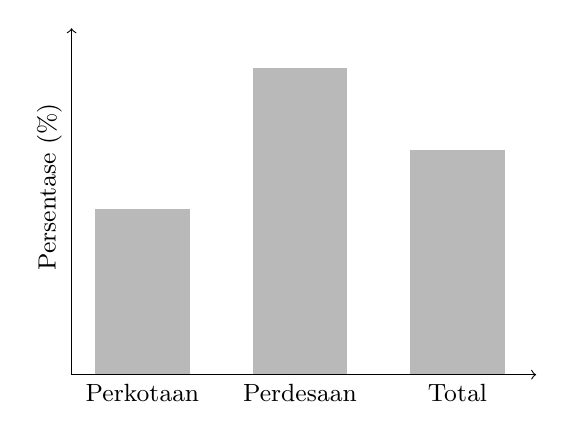
\begin{tikzpicture}
  \foreach \x/\h/\lbl in {0/2.1/Perkotaan, 2/3.9/Perdesaan, 4/2.85/Total} {
    \fill[gray!55] (\x,0) rectangle (\x+1.2,\h);
    \node[below] at (\x+0.6,0) {\small \lbl};
  }
  \draw[->] (-0.3,0) -- (5.6,0);
  \draw[->] (-0.3,0) -- (-0.3,4.4) node[above,rotate=90,anchor=south west,xshift=-3.2cm]{\small Persentase (\%)};
\end{tikzpicture}}%
\usebox\skripsiblokbox\par
\addvspace{0.15\sjudul}
% Sumber: tepat di TEPI KIRI gambar, diletakkan SEBELUM judul (pedoman).
\parbox[t]{\wd\skripsiblokbox}{\raggedright\setlength{\parindent}{0pt}\small Sumber: diolah dari Tabel~\ref{tab:miskin} (data ilustrasi)}\par
% Judul gambar: di BAWAH gambar/sumber, DIPUSATKAN (center).
\caption{Persentase penduduk miskin menurut daerah}
\label{gbr:bar}
\end{figure}

Berdasarkan Gambar~\ref{gbr:bar}, persentase kemiskinan di perdesaan lebih tinggi
dibandingkan perkotaan.

\section{Contoh Tabel Lebar (Orientasi \emph{Landscape})}
Tabel yang terlalu lebar untuk orientasi potret dapat disajikan pada halaman
\emph{landscape}, atau diperkecil hingga ukuran huruf minimal 8 pt (pedoman).
Tabel~\ref{tab:lebar} menyajikan contoh tabel lebar berorientasi \emph{landscape};
judul tetap di batas kiri teks (kiri halaman \emph{landscape}) dan sumber di
bawah-kiri, sedangkan tabel diletakkan di tengah.

\begin{landscape}
\begin{table}[H]
\centering
\caption{Contoh tabel lebar berorientasi landscape dengan banyak kolom (data ilustrasi)}
\label{tab:lebar}
\sbox\skripsiblokbox{\begin{tabular}{|l|r|r|r|r|r|r|r|r|}
\hline
\textbf{Provinsi} & \textbf{2018} & \textbf{2019} & \textbf{2020} & \textbf{2021} & \textbf{2022} & \textbf{2023} & \textbf{2024} & \textbf{2025} \\ \hline
\multicolumn{1}{|c|}{(1)} & \multicolumn{1}{c|}{(2)} & \multicolumn{1}{c|}{(3)} & \multicolumn{1}{c|}{(4)} & \multicolumn{1}{c|}{(5)} & \multicolumn{1}{c|}{(6)} & \multicolumn{1}{c|}{(7)} & \multicolumn{1}{c|}{(8)} & \multicolumn{1}{c|}{(9)} \\ \hline
Aceh        & 15,68 & 15,32 & 14,99 & 15,33 & 14,75 & 14,45 & 14,23 & 13,98 \\
Sumatera Utara & 8,94 & 8,83 & 8,75 & 9,01 & 8,42 & 8,15 & 7,99 & 7,80 \\
Jawa Barat  & 7,25 & 6,91 & 7,88 & 8,40 & 7,98 & 7,62 & 7,41 & 7,20 \\
Jawa Tengah & 11,32 & 10,80 & 11,41 & 11,79 & 10,93 & 10,77 & 10,51 & 10,30 \\
DI Yogyakarta & 11,81 & 11,44 & 12,28 & 11,91 & 11,49 & 11,04 & 10,83 & 10,62 \\ \hline
\end{tabular}}%
\usebox\skripsiblokbox\par
\addvspace{0.2\baselineskip}
\parbox[t]{\wd\skripsiblokbox}{\raggedright\setlength{\parindent}{0pt}\small Sumber: Badan Pusat Statistik (data ilustrasi)}
\end{table}
\end{landscape}

  \chapter{Kesimpulan dan Saran}
\emph{Cara menulis bab ini.} Bab Kesimpulan dan Saran berisi jawaban ringkas atas rumusan masalah (Kesimpulan) dan rekomendasi tindak lanjut (Saran). Tidak memuat angka/tabel baru.


\section{Kesimpulan}
\emph{Cara menulis.} Tulis kesimpulan sebagai jawaban langsung dan ringkas atas tiap rumusan masalah, paralel dengan tujuan penelitian, tanpa tabel/angka/kutipan baru.

Bagian ini memuat kesimpulan yang menjawab tujuan penelitian secara ringkas dan
tegas, tanpa mengulang seluruh pembahasan.

\section{Saran}
\emph{Cara menulis.} Berikan saran yang konkret dan dapat ditindaklanjuti (pengembangan keilmuan, penerapan praktis, serta penelitian selanjutnya).

Bagian ini memuat saran, antara lain:
\begin{enumerate}[leftmargin=*]
  \item rekomendasi pengembangan metode atau model;
  \item usulan penelitian lanjutan yang relevan.
\end{enumerate}

\fi

% ===================== DAFTAR PUSTAKA ========================
\begingroup
\singlespacing                 % daftar pustaka 1 spasi di dalam entri
\setlength{\bibitemsep}{0.5\baselineskip}  % jarak antar-entri ~1,5 spasi
\printbibliography[heading=bibintoc,title={DAFTAR PUSTAKA}]
\endgroup

% ======================== LAMPIRAN ==========================
% ---------- LAMPIRAN ----------
% Judul "LAMPIRAN" sebagai bab tak bernomor; tiap lampiran didaftarkan via
% \lampiran{Judul} agar muncul di Daftar Lampiran.
\judulfrontmatter{Lampiran}{LAMPIRAN}

\lampiran{Daftar Perintah/Kode yang Digunakan}
\noindent\textbf{Lampiran 1. Daftar Perintah/Kode yang Digunakan}
\vspace{0.3cm}

Lampiran memuat materi pendukung yang terlalu panjang untuk badan teks, misalnya
potongan kode, kuesioner, atau tabel rinci. Potongan kode disajikan dengan
lingkungan \texttt{lstlisting} (baris yang panjang otomatis dilipat):

\begin{lstlisting}[language=R]
# Contoh kode R: estimasi model proxy means test dengan validasi silang
library(caret)
set.seed(123)
kontrol <- trainControl(method = "cv", number = 10)
model <- train(log_pengeluaran ~ ., data = rumah_tangga, method = "ranger", trControl = kontrol, importance = "permutation")
print(model$results)
\end{lstlisting}

\lampiran{Output Tambahan}
\noindent\textbf{Lampiran 2. Output Tambahan}
\vspace{0.3cm}

Isi lampiran kedua.


% ===================== RIWAYAT HIDUP ========================
% ---------- RIWAYAT HIDUP ----------
\judulfrontmatter{Riwayat Hidup}{RIWAYAT HIDUP}

\noindent\justifying
\skNama\ lahir di [kota] pada [tanggal]. Penulis menyelesaikan pendidikan
[riwayat pendidikan] dan diterima di Politeknik Statistika STIS pada tahun [tahun].
Selama masa studi, penulis aktif dalam [kegiatan]. Skripsi berjudul
``\skJudul'' merupakan salah satu syarat untuk memperoleh sebutan Sarjana Terapan
Statistika.


\end{document}
